\documentclass[notitlepage, a4paper, 11pt]{article}

\usepackage{geometry}
\geometry{
	a4paper,
	total={170mm,257mm},
	left=20mm,
	top=20mm,
}

\usepackage{xcolor}
\usepackage{graphicx}
\usepackage{amsmath}
\usepackage{listings}
\usepackage{xcolor}
\usepackage{minted}
\usepackage{tikz}
\usepackage[european resistors]{circuitikz}
\usepackage{caption}
\usepackage{subcaption}
\usepackage{hyperref}
\hypersetup{
	pdfborder = false,
	colorlinks=true,
	linkcolor=black,
	filecolor=black,      
	urlcolor=blue,
	pdftitle={Overleaf Example},
	pdfpagemode=FullScreen,
}
\title{Fourier Series\\
	\large Laboratory II}
\author{Patrycja Nazim, Adrian Król, Kamil Chaj}
\date{}

\begin{document}
	\maketitle
	\section{Aim of the exercise}
	The purpose of exercise was to experimentally familiarize with the Fourier series - an operation
	that allows to represent any real periodic signal by the sum of sinusoidal signals. We measured the signals generated by the independent function generator with a vector spectrum analyzer.
	
	\section{What is Fourier Series}
	A Fourier series is an expansion of a periodic function $f(x)$ in terms of an infinite sum of sines and cosines. Fourier series make use of the orthogonal relationships of the sine and cosine functions. The computation and study of Fourier series is known as harmonic analysis and is extremely useful to break up an arbitrary periodic function into a set of simple terms that can be plugged in, solved individually, and then recombined to obtain the solution to the original problem or an approximation to it to whatever accuracy is desired or practical
	
	\section{Course of measurements}
	During our measurements we skipped first part of exercise and measured all signals in configuration for second part (Fig. \ref{fig:Measurements configuration}).
	
	\begin{figure}[H]
		\centering
		\begin{circuitikz}[scale = 0.7, transform shape]
			\ctikzset{bipoles/oscope/width=1.5}
			\ctikzset{bipoles/oscope/height=1}
			\draw (2, 3.5) node[oscopeshape](O) {Oscilloscope};
			\draw [black, thick] (-2.5, 1) rectangle (-0.5, 2.5);
			\draw [black, thick] (6.5, 1) rectangle (4.5, 2.5);
			\draw [black, thick] (0, 0) rectangle (4, 2);
			\draw (-1, 1.75) node[bnc, font=\tiny](CH1) {CH1};
			\draw (5, 1.4) node[bnc, xscale=-1, font=\tiny](INPUT2) {\ctikzflipx{INPUT2}};
			\draw (5, 2.1) node[bnc, xscale=-1, font=\tiny](INPUT1) {\ctikzflipx{INPUT1}};
			\draw (0.5, 1) node[bnc, xscale=-1, font=\tiny](CONX1) {\ctikzflipx{CONX1}};
			\draw (3.5, 1) node[bnc, font=\tiny](CONX2) {CONX2};
			\draw (O.in 1) node[bnc, anchor=zero, rotate=-90](IN1) {};
			\draw (O.in 2) node[bnc, anchor=zero, rotate=-90](IN2) {};
			\draw (CH1.hot) to[short, -*] (-0.3, 1.75) -- (-0.3, 1) -- (CONX1.hot);
			\draw (-0.3, 1.75) to[short] (-0.3, 2.25) to[short, -*] (1.57, 2.25) -- (IN1.hot);
			\draw (1.57, 2.25) to[short] (4.25, 2.25) -- (4.25, 2.1) -- (INPUT1.hot);
			\draw (INPUT2.hot) to[short, -*] (4.25, 1.4) -- (4.25, 1) -- (CONX2.hot);
			\draw (4.25, 1.4) -- (4.25, 1.6) -- (2.42, 1.6) -- (IN2.hot);
			\node [black] at (2, 0.5) {RC Filters};
			\node [black, above] at (-1.5, 2.5) {\small Function Generator};
			\node [black, above] at (5.5, 2.5) {\small Spectrum Analyzer};
		\end{circuitikz}
		\caption{Measurements configuration}
		\label{fig:Measurements configuration}
	\end{figure}
	
	After connecting Function Generator, Spectrum Analyzer, Oscilloscope and board with RC filters according to above configuration (Fig. \ref{fig:Measurements configuration}) we set Function Generator to Amplitude to $V_{pp}$ = 5V and Frequency 1 kHz. 
	With everything set up we proceeded with exercise and recording output of Oscilloscope and Spectrum Analyzer for signals:
	\begin{itemize}
		\setlength\itemsep{0.1em}
		\item Sin wave
		\item Square wave 50\% duty cycle
		\item Square wave 25\% duty cycle
		\item Triangle wave 50\% symmetry ratio
		\item Triangle wave 40\% symmetry ratio
	\end{itemize}
	For Square wave 50\% duty cycle and Triangle wave 40\% symmetry ratio we also recorded Response for both RC Circuits (Fig. \ref{fig: Circuit})
	
	\begin{figure}[H]
		\centering
		\begin{subfigure}{0.45\textwidth}
			\centering
				\begin{circuitikz}[scale = 0.7, transform shape]
				\draw (0,0) node[bnc](B1) {}
				to[R, l=$R_{11}$, a=1.5k$\Omega$] (3,0)
				to[C, l=$C_{11}$, a=47nF] (3,-2)
				node[ground] {}
				;
				\draw (3,0) 
				to[short] (4.5,0)
				node[bnc, xscale=-1](B2){\scalebox{-1}[1]{}}
				;
				\draw node[ground] at (B1.shield) {};
				\draw node[ground] at (B2.shield) {};
			\end{circuitikz}
			\caption{Circuit A}
			\label{fig:Circuit A}
		\end{subfigure}
		\begin{subfigure}{0.45\textwidth}
			\centering
				\begin{circuitikz}[scale = 0.7, transform shape]
				\draw (0,0) node[bnc](B1) {}
				to[R, l=$R_{11}$, a=1.5k$\Omega$] (3,0)
				to[C, l=$C_{11}$, a=47nF] (3,-2)
				node[ground] {}
				;
				\draw (3,0) 
				to[short] (4.5,0)
				node[bnc, xscale=-1](B2){\scalebox{-1}[1]{}}
				;
				\draw node[ground] at (B1.shield) {};
				\draw node[ground] at (B2.shield) {};
			\end{circuitikz}
			\caption{Circuit B}
			\label{fig:Circuit B}
		\end{subfigure}
		\caption{Measured RC Circuits}
		\label{fig: Circuit}
	\end{figure}
	
	\section{Method for calculating Fourier Series coefficients}
	
	\section{measurements vs calculations}
	\begin{center}
		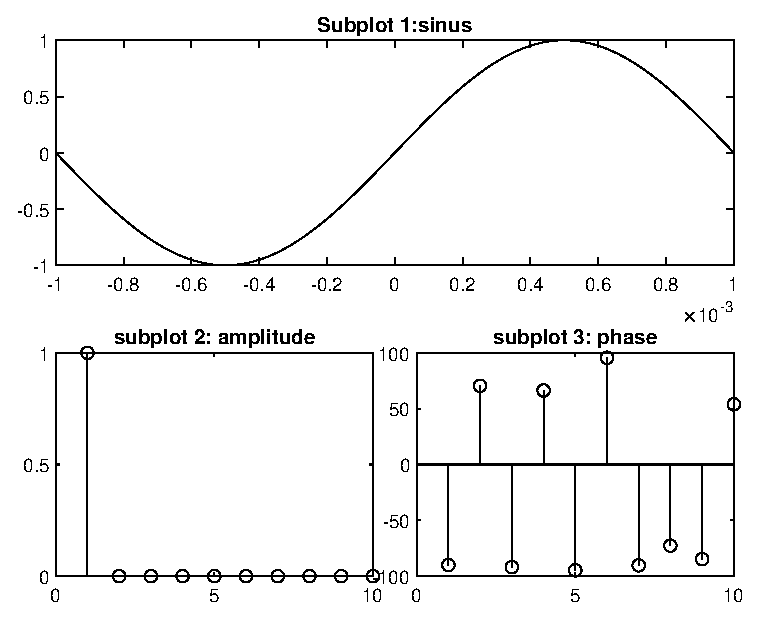
\includegraphics{../Matlab/img/sin}
		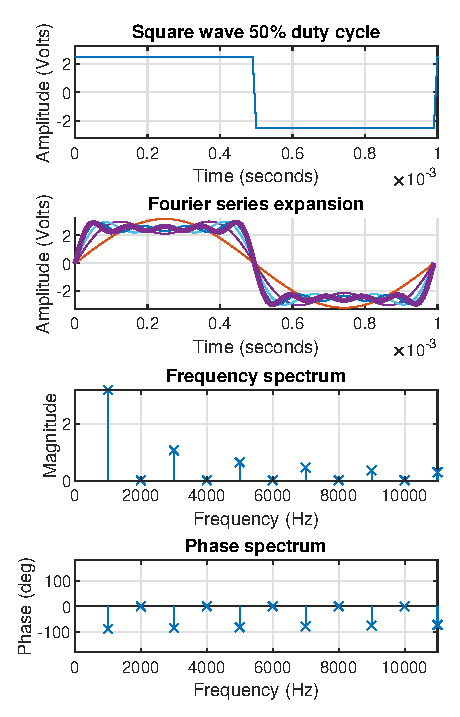
\includegraphics{../Matlab/img/sqr50}
		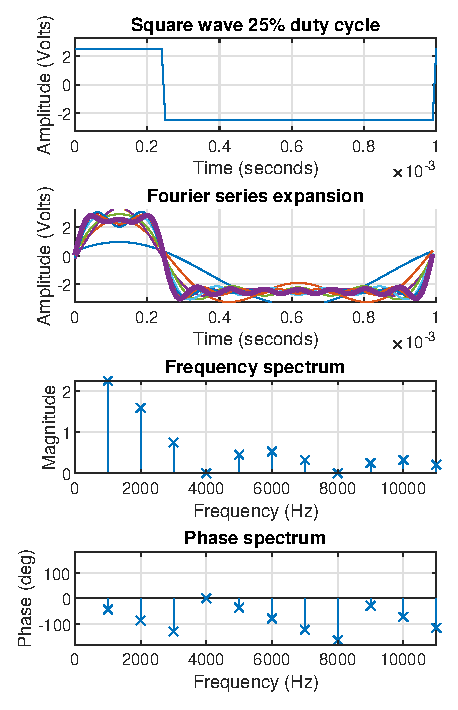
\includegraphics{../Matlab/img/sqr25}
		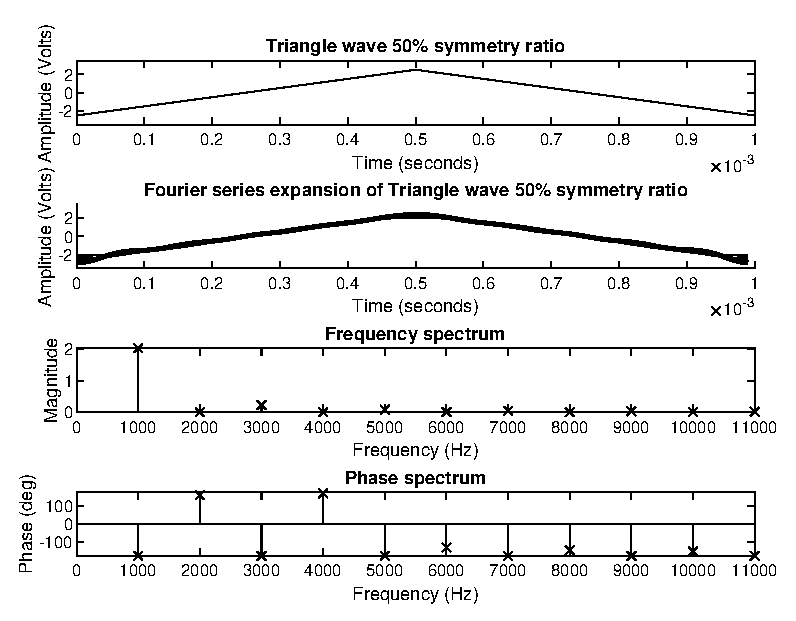
\includegraphics{../Matlab/img/tri50}
		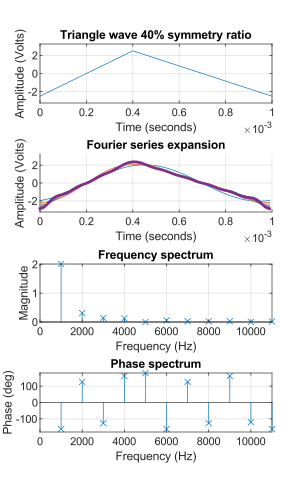
\includegraphics{../Matlab/img/tri40}
	\end{center}
	
	\newpage
	\appendix
	\section{Source Code}\label{sec:source-code}
	\href{https://github.com/kamilix2003/CT_labs}{GITHUB repository}
	\subsection*{Fourier.m}
	\inputminted{matlab}{../Matlab/Fourier.m}
	\subsection*{fourier coefficient.m}
	\inputminted{matlab}{../Matlab/fourier_coefficient.m}
	\subsection*{RC circuit.m}
	\inputminted{matlab}{../Matlab/RC_circuit.m}
\end{document}